% Phụ lục A

\chapter{Các chỉ số đánh giá} % Tên của phụ lục

\label{AppendixA} % Để trích dẫn chương này ở chỗ nào đó trong bài, hãy sử dụng lệnh \ref{AppendixA} 

%----------------------------------------------------------------------------------------
\section*{I. Đánh giá mô hình Phát hiện đối tượng}

Trong bài toán này, hiệu suất mô hình được xác định dựa trên sự tương quan về vị trí không gian giữa hộp dự đoán và hộp thực tế.

\subsection*{1. Chỉ số IoU}
Chỉ số này đo lường mức độ trùng khớp về mặt không gian giữa hai vùng ảnh.
\begin{equation}
IoU = \frac{Area(B_{pred} \cap B_{gt})}{Area(B_{pred} \cup B_{gt})}
\end{equation}
\textbf{Trong đó :}
\begin{itemize}
    \item $B_{pred}$: Hình hộp giới hạn (\textit{Bounding Box}) do mô hình dự đoán.
    \item $B_{gt}$: Hình hộp giới hạn thực tế (\textit{Ground Truth}) do người gán nhãn.
    \item $Area(B_{pred} \cap B_{gt})$: Diện tích vùng giao nhau giữa hộp dự đoán và hộp thực tế.
    \item $Area(B_{pred} \cup B_{gt})$: Tổng diện tích bao phủ của cả hai hộp giới hạn.
\end{itemize}

\subsection*{2. Precision}
Đo lường tỉ lệ dự đoán đúng trong số tất cả các dự đoán mà mô hình đưa ra.
\begin{equation}
Precision = \frac{TP}{TP + FP}
\end{equation}
\textbf{Trong đó :}
\begin{itemize}
    \item $TP$ (\textit{True Positive}): Số lượng đối tượng dự đoán đúng.
    \item $FP$ (\textit{False Positive}): Số lượng đối tượng dự đoán sai (nhận nhầm bối cảnh là đối tượng).
\end{itemize}

\subsection*{3. Recall}
Đo lường tỉ lệ đối tượng được tìm thấy trên tổng số đối tượng thực tế tồn tại.
\begin{equation}
Recall = \frac{TP}{TP + FN}
\end{equation}
\textbf{Trong đó :}
\begin{itemize}
    \item $TP$ (\textit{True Positive}): Số lượng đối tượng dự đoán đúng.
    \item $FN$ (\textit{False Negative}): Số lượng đối tượng thực tế bị mô hình bỏ sót.
\end{itemize}

\subsection*{4. Average Precision}
Đại diện cho hiệu năng của mô hình trên một lớp đối tượng cụ thể thông qua đường cong Precision-Recall.
\begin{equation}
AP = \int_0^1 P(R)\, dR
\end{equation}
\textbf{Trong đó :}
\begin{itemize}
    \item $R$: Chỉ số Recall.
    \item $P(R)$: Giá trị Precision tương ứng với từng mức độ Recall trên đồ thị.
\end{itemize}

\subsection*{5. Mean Average Precision}
Giá trị trung bình của AP trên tất cả các lớp đối tượng cần nhận diện.
\begin{equation}
mAP = \frac{1}{C} \sum_{c=1}^{C} AP_c
\end{equation}
\textbf{Trong đó :}
\begin{itemize}
    \item $C$: Tổng số lớp (classes) đối tượng trong tập dữ liệu.
    \item $AP_c$: Giá trị Average Precision của lớp thứ $c$.
\end{itemize}

\begin{figure}[H]
    \centering
    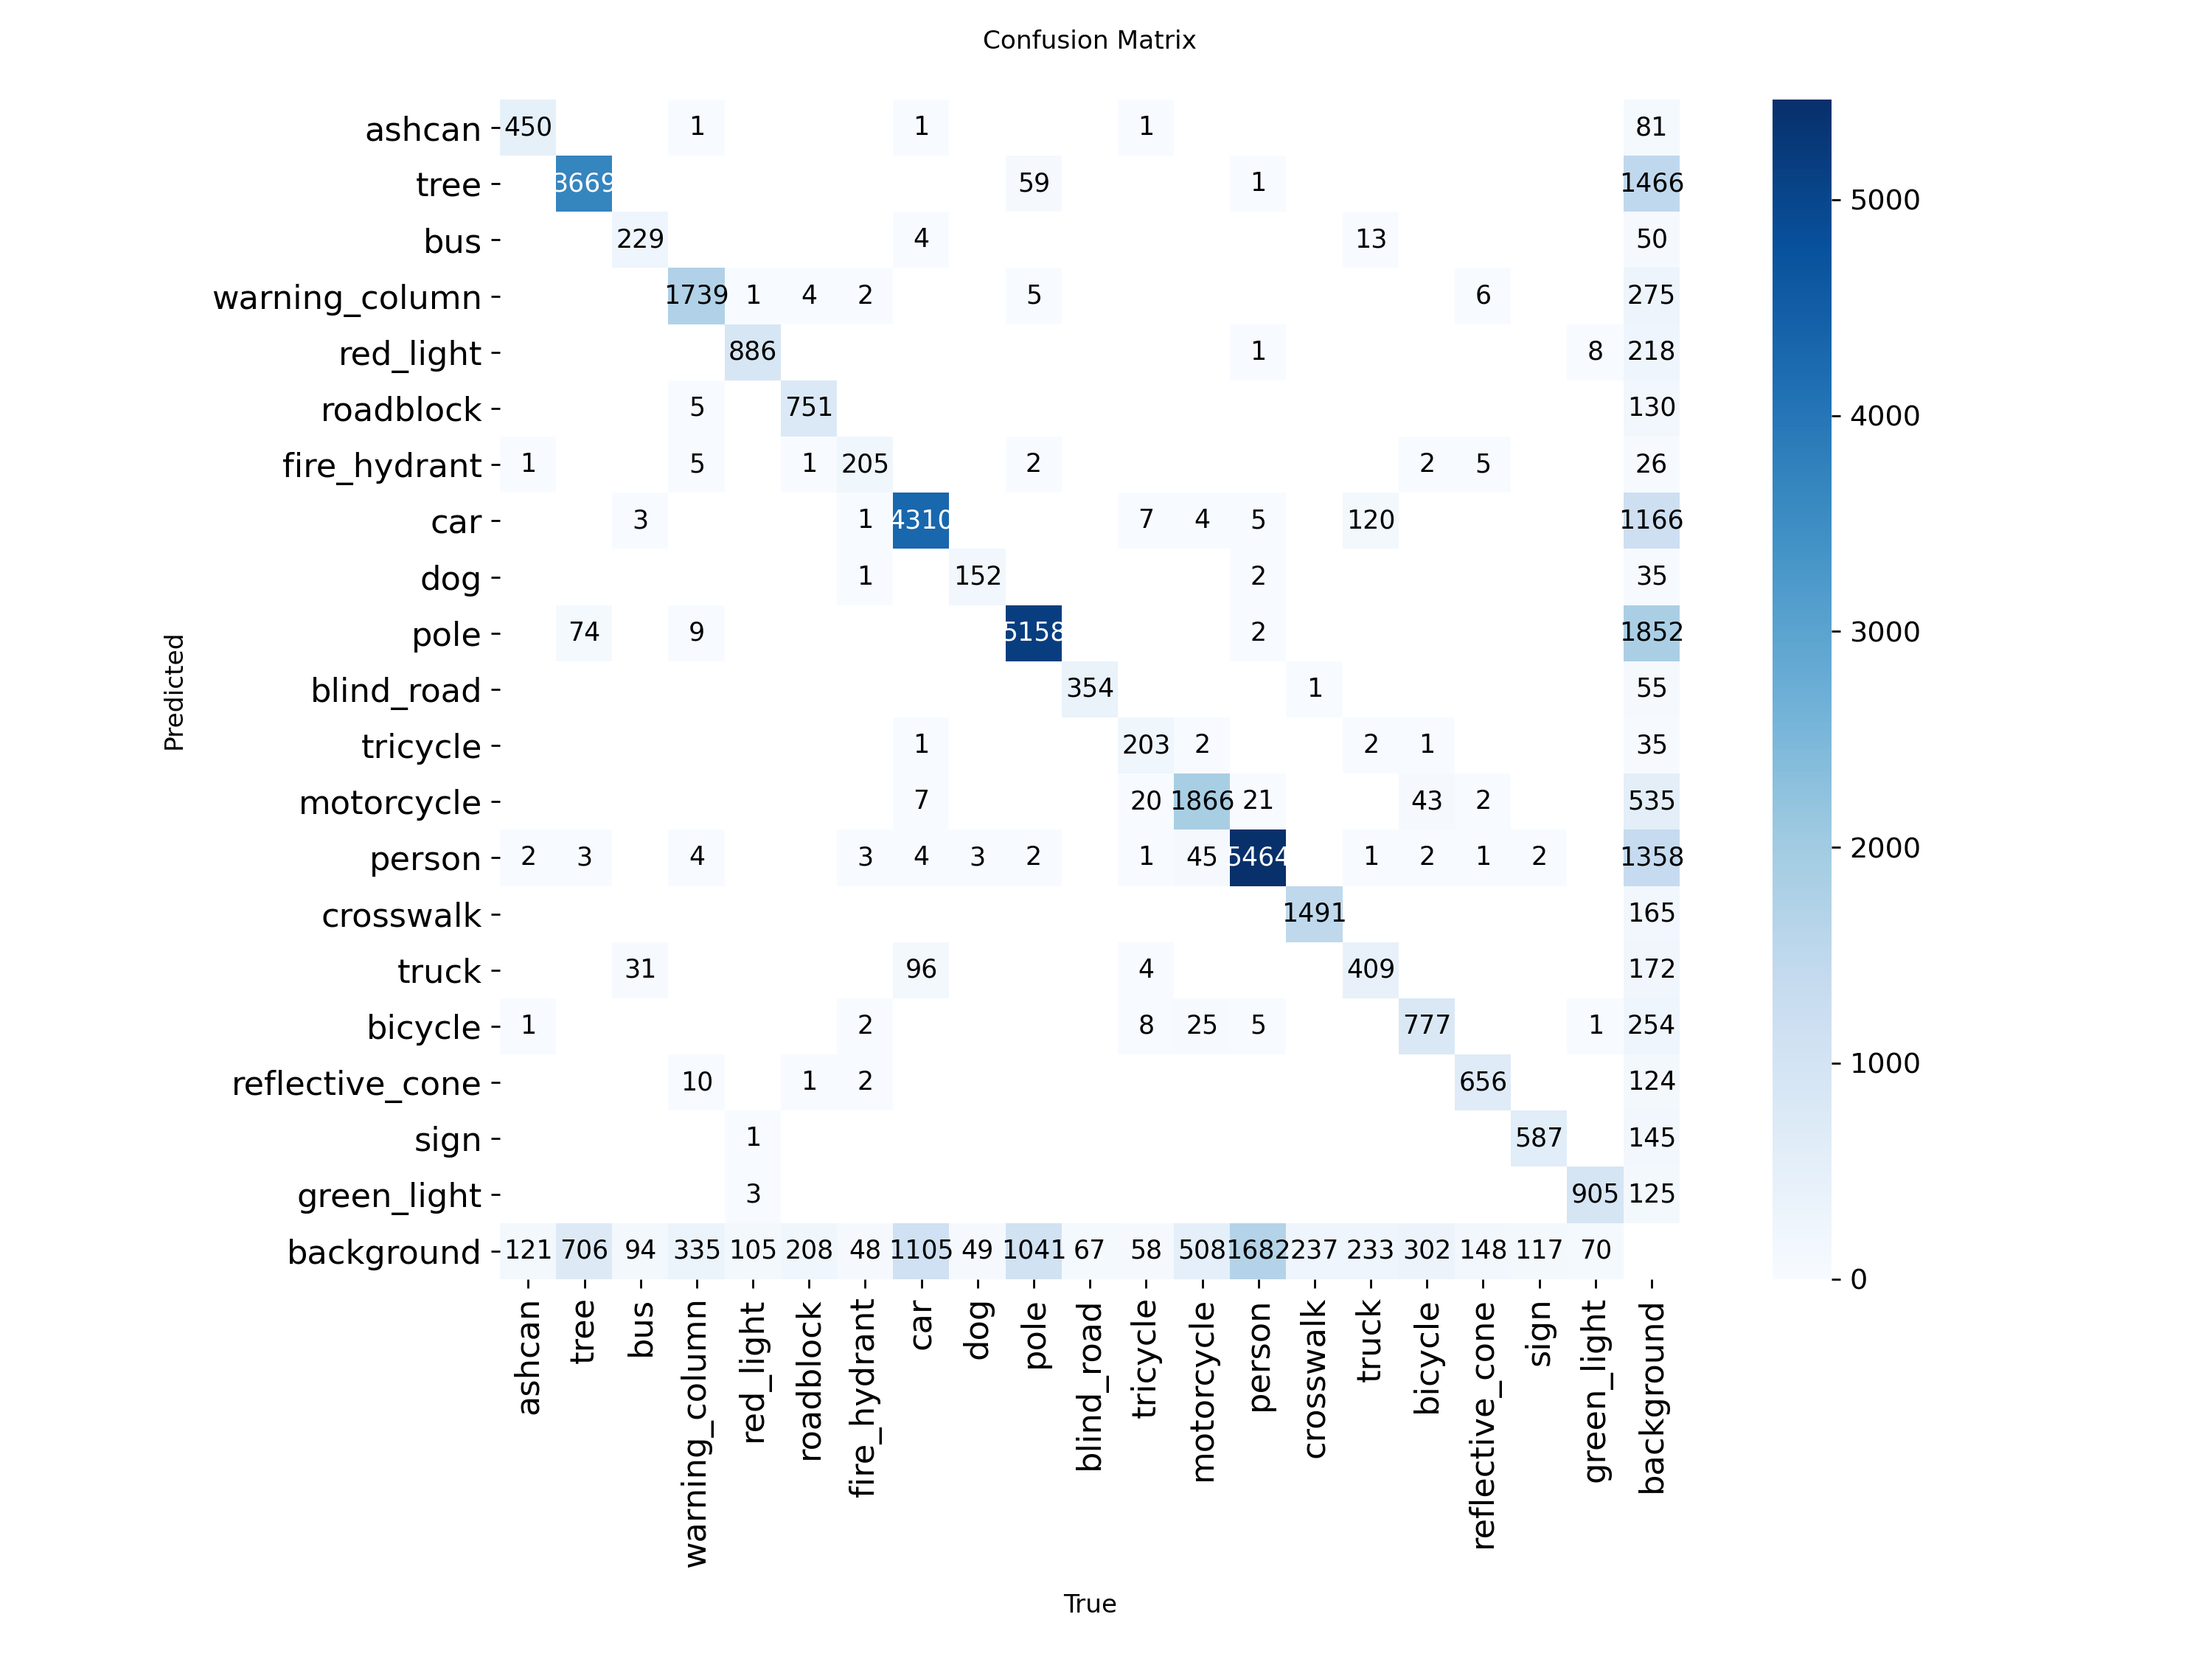
\includegraphics[width=1.1\linewidth]{Figures/Chapter3/confusion_matrix.png}
    \caption{Ma trận nhầm lẫn theo từng thuộc tính}
    \label{fig:matran}
\end{figure}


\subsection*{2. Các chỉ số đánh giá tầng ước tính chiều sâu (MiDAS)}

Để kiểm thử sai số cự ly giữa khoảng cách thực tế thu thập tại hiện trường và điểm số chiều sâu trích xuất từ mô hình lai, hệ thống áp dụng hai chỉ số toán học sau:

\begin{equation}
MAE = \frac{1}{N} \sum_{i=1}^{N} \left| d_i - \hat{d}_i \right|
\end{equation}

\begin{equation}
Rel\,RMSE = \sqrt{\frac{1}{N} \sum_{i=1}^{N} \left( \frac{d_i - \hat{d}_i}{d_i} \right)^2}
\end{equation}

Trong đó:
\begin{itemize}
    \item $N$: Tổng số mẫu hộp bao chướng ngại vật được đưa vào kiểm thử cự ly.
    \item $d_i$: Khoảng cách thực tế đo đạc bằng thước dây/cảm biến chuẩn của vật cản thứ $i$ (tính bằng mét).
    \item $\hat{d}_i$: Giá trị chiều sâu tương ứng do hệ thống tính toán (Giá trị điểm số \textit{score} đại diện sau khi tính phân vị thứ 80 trong vùng ma trận cắt từ \texttt{depth\_map} của mô hình \textit{MiDAS\_small}).
\end{itemize}

Để đánh giá toàn diện hiệu năng của mô hình, nhóm đã tiến hành thực nghiệm trên tập mẫu thử nghiệm gồm 400 trường hợp cụ thể. Tập mẫu này được chia đều thành 4 nhóm khoảng cách cảnh báo (bao gồm: Rất gần, Gần, Trung bình, và Xa), tương ứng với 100 lần thử nghiệm cho mỗi nhóm. Kết quả phân lớp chi tiết và mức độ sai lệch giữa các phân khúc được thống kê cụ thể thông qua bảng ma trận nhầm lẫn ở Hình \ref{tab:depth_confusion_matrix}.

\begin{table}[H]
\centering
\caption{Ma trận nhầm lẫn kết quả phân lớp khoảng cách cảnh báo của MiDaS.}
\label{tab:depth_confusion_matrix}
\renewcommand{\arraystretch}{1.25} % Giúp các hàng thoáng và đẹp hơn
\setlength{\tabcolsep}{10pt}       % Nới rộng khoảng cách giữa các cột

\begin{tabular}{llcccc}
\toprule
 & & \multicolumn{4}{c}{\textbf{Khoảng cách Thực tế (Ground Truth)}} \\ 
\cmidrule(lr){3-6}
 & & \textbf{Rất gần} & \textbf{Gần} & \textbf{Trung bình} & \textbf{Xa} \\ 
\midrule
\multirow{4}{*}{\textbf{\begin{tabular}[c]{@{}l@{}}Hệ thống\\ Dự đoán\end{tabular}}} 
 & \textbf{Rất gần}   & \textbf{94} & 5           & 0           & 0  \\ 
 & \textbf{Gần}       & 6           & \textbf{88} & 7           & 0  \\ 
 & \textbf{Trung bình} & 0           & 7           & \textbf{85} & 9  \\ 
 & \textbf{Xa}        & 0           & 0           & 8           & \textbf{91} \\ 
\bottomrule
\end{tabular}
\end{table}